\documentclass[12pt]{article}

\usepackage{amsmath}
\usepackage{graphicx}
\begin{document}



\begin{center}
{\Huge \bf Assignment 1}\\
\end{center}
\hrulefill\\
\begin{large}
\bf Name:-Pawan Jagannath Aru\\
\bf MIS no- 112103013\\
\bf Subject:- DTL LAB\\
\bf Division:-1\\
\bf Batch:-S1\\
\bf \date{today}
\end{large}
\hrule
\pagenumbering{gobble}
\pagenumbering{arabic}
\tableofcontents

\newpage
\section{Coep}
\subsection{About}
\begin{figure}[h]                %h is used to force image to place as given.
    \centering
    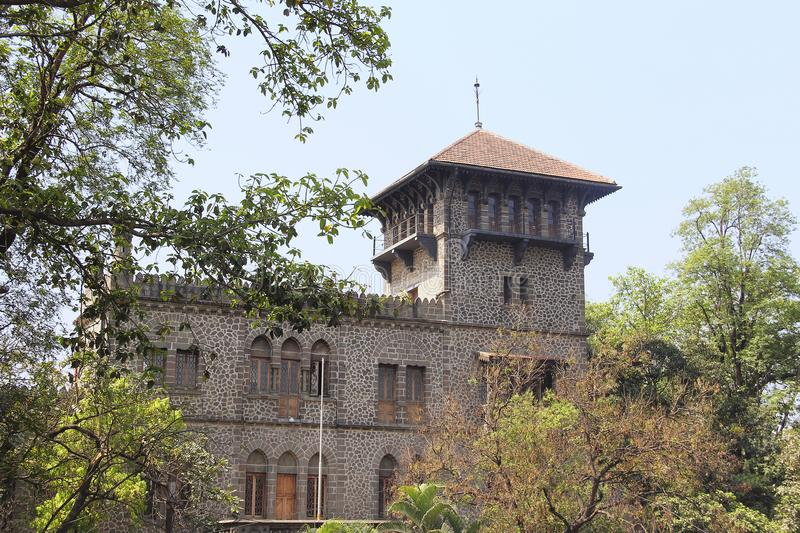
\includegraphics[scale=1]{coepcollege}
    \caption{Coep College}
    \label{fig:coep1}
\end{figure}

College of Engineering, Pune (CoEP),as shown in \ref{fig:coep1} chartered in 1854 is a nationally respected leader in technical education. The institute is distinguished by its commitment to finding solutions to the great predicaments of the day through advanced technology. The institute has a rich history and dedication to the pursuit of excellence. CoEP offers a unique learning experience across a spectrum of academic and social experiences. With a firm footing in truth and humanity, the institute gives you an understanding of both technical developments and the ethics that go with it. The curriculum is designed to enhance your academic experience through opportunities like internships, study abroad programmes and research facilities.\\ 
\hrule
\subsection{Clubs}
\begin{enumerate}
\item Boat Club
\item Bhau Ecell Club
\item Science Club
\item Coep CSI Chapter club
\end{enumerate}

\section{Clubs}
\hrulefill
\subsection{Boat Club}
\begin{figure}[h]
    \centering
    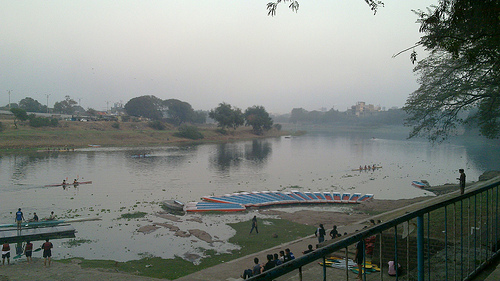
\includegraphics[scale=0.5]{boatclub}
    \caption{Boat club}
    \label{fig2:boatclub}
\end{figure}
\noindent The Boatclub, as it is known, is one of the favourite spot for most people in college. The riverside ambience offers a majestic view of the Mula River. The Boatclub has become synonymous with COEP for every COEPian.\\
COEP is proud to have a Boat Club, which is one of its kind in the country. Situated on the banks of Mula River, this club was established in the year 1928. The club owns about 70 trainee and racing boats, which can be used for various competitions besides regular practice. The club is an active member of professional associations like Maharashtra Rowing Association (MRA) and the Amateur Rowers Association (ARAE).\\
\hrule
\subsection{Bhau Ecell Club}
\begin{figure}[h]
   \centering
   
\includegraphics[scale=5]{bhaus ecell logo}
   \caption{Bhau's Ecell Club}
   \label{fig3:bhaucell}
\end{figure}
BHAUs Innovation and Entrepreneurship Cell is a students led club, supported by the institute and mentored by faculty. BHAUs Innovation and Entrepreneurship Cell, COEP aims to foster a culture of entrepreneurship among students. The cell has been organizing various engaging events to inculcate an interest in entrepreneurship and start-ups. For example, IDEA competition, B-Plan Competition, Case Study Activity, Budgeting, Workshops, and seminars, etc. COEP's IE-Cell is a pre-incubation center of COEP and thus provides mentoring to the students having ideas or innovations and helping them follow steps like ideation, innovation, proof of concept, business model, prototyping, designing. Various innovation and entrepreneurship related activities are conducted as recommended by MoE' s (Ministry of Education) Innovation Cell under the guidance of industry experts, alumni, director COEP, patent attorney, and experts from incubators.\\
\hrule
\subsection{Science Club}
\begin{figure}[h]
    \centering
    
\includegraphics[scale=0.4]{science club}
    \caption{Science club}
    \label{fig4:scienceclub}
\end{figure}
The Science club, nurturing innovation and raising the profile of science through activities and workshops has conjured up a lot of interest amongst the students of COEP. Science rules the world and human beings attempt to understand its mysterious ways by making laws and theories. We at the science club, aim to encourage scientific temper and answer the burning questions that drive students to pursue research into unknown frontiers.\\
The club strives to quench a student’s thirst for science by organizing various exciting events such as demonstration experiments, science quizzes, talks and lectures by eminent scientists from all over the globe, visits to various labs, workshops and much more.\\
\hrule
\subsection{CSI Chapter Club}
\begin{figure}[h]
    \centering
    
\includegraphics[scale=0.5]{csi logo}
    \caption{CSI computer society}
    \label{fig4:csilogo}
\end{figure}
The Computer Society of India (CSI) Student Chapter of College of Engineering Pune (COEP) Tech, established in October 2018 is an active student organization which organizes a number of technical activities including workshops, competitions, technical symposiums, guest lectures etc. for its student members. Under the guidance of Department of Computer Engineering and Information Technology COEP Tech, the student chapter has over 300 members and is run by a Core Team and faculty from the department.CSI COEP Tech Student Chapter gives students the opportunity to grow in the field of IT.



\clearpage

\end{document}